\documentclass[12pt]{article}
\usepackage[brazil]{babel}
\usepackage[utf8]{inputenc}
\usepackage{amsmath}
\usepackage{amsfonts}
\usepackage{amssymb}
\usepackage{geometry}
\usepackage{graphicx}
\usepackage{float}
\usepackage{enumitem}
\usepackage{multicol}
\usepackage{array}
\usepackage{xcolor}
\usepackage[T1]{fontenc}
\usepackage{setspace}

\newif\ifmostravermelho
%\mostravermelhofalse %começa falso

\newcommand{\vermelho}[1]{%
  \ifmostravermelho
    {\color{red}#1}%
  \else
    #1%
  \fi
}

%\newcommand{\vermelho}[1]{{\color{red}#1}}
\geometry{a4paper, margin=1.2cm}
\setlength{\parindent}{1.2cm}

% implementa contador
% Definindo o contador e o comando de questão
\newcounter{questao}
\newcommand{\novaquestao}[1]{%
  \stepcounter{questao}%
  \subsection*{Questão \thequestao\ (#1)}%
}

\begin{document}
    \large
    \onehalfspacing
    % Cabeçalho reduzido
    \vspace{0.5cm}
    \begin{center}
        \resizebox{\textwidth}{!}{%
        \begin{tabular}{|l l|}
            \hline
            \textbf{ESCOLA:} & EETI GILBERTO MESTRINHO DE MEDEIROS RAPOSO \\
            \textbf{ALUNA(O):} & \underline{\hspace{7cm}} \textbf{SÉRIE:} \underline{\hspace{1.5cm}} \textbf{TURMA:} \underline{\hspace{1.5cm}} \\
            \textbf{PROFESSOR:} & \underline{\hspace{7cm}} \textbf{DATA:} \underline{\hspace{1.5cm}}/\underline{\hspace{1.5cm}}/\underline{\hspace{1.5cm}} \\
            \textbf{VALOR:} & \underline{\hspace{3cm}} \textbf{NOTA:} \underline{\hspace{1.5cm}} \\
            \hline
        \end{tabular}
        }
    \end{center}
    \vspace{0.5cm}
    
    % Título manual
    \begin{center}
        \Large\textbf{Lista - Introdução à Probabilidade}
    \end{center}
    
    \vspace{0.3cm}
    
    \section*{\vermelho{ATENÇÃO}}

    \begin{itemize}[noitemsep, after=\vspace{0.5\baselineskip}]
        \item Resolva toda a lista, justificando cada questão.
        \item Colocar o nome completo e identificação no cabeçalho.
        \item Faça na lista, se e somente se a resolução de cada questão couber em cada questão.
        \item Há apenas uma opção correta em cada questão de múltipla escolha.
        \item Caso opte por fazer numa folha à parte, identifique cada questão.
    \end{itemize}
    

    % Início das colunas com linha vertical
    %\mostravermelhotrue
    \begin{multicols}{2}
        \raggedcolumns
        
        \novaquestao{Enem 2015}
            Em uma central de atendimento, cem pessoas receberam senhas numeradas de 1 até 100. 
            Uma das senhas é sorteada ao acaso. Qual é a probabilidade de a senha sorteada ser um 
            número de 1 a 20?
            
            \begin{enumerate}[label=(\alph*), noitemsep]
                \item {1}/{100}
                \item {19}/{100}
                \item {20}/{100} %
                \item {21}/{100} 
                \item {80}/{100}
            \end{enumerate}

        \novaquestao{Enem 2023}

            No alojamento de uma universidade, há alguns quartos com o padrão superior ao 
            dos demais. Um desses quartos ficou disponível, e muitos estudantes se candidataram
            para morar no local. Para escolher quem ficará com o quarto, um sorteio será 
            realizado. Para esse sorteio, cartões individuais com os nomes de todos os 
            estudantes inscritos serão depositados em uma urna, sendo que, para cada estudante
            de primeiro ano, será depositado um único cartão com seu nome; para cada estudante
            de segundo ano, dois cartões com seu nome; e, para cada estudante de terceiro ano,
            três cartões com seu nome. Foram inscritos 200 estudantes de primeiro ano, 150 de 
            segundo ano e 100 de terceiro ano. Todos os cartões têm a mesma probabilidade de 
            serem sorteados. Qual a probabilidade de o vencedor do sorteio ser um estudante 
            de terceiro ano?

            \begin{enumerate}[label=(\alph*), noitemsep]
                \item {1}/{2}
                \item {1}/{3}
                \item {1}/{8}
                \item {2}/{9}
                \item {3}/{8}
            \end{enumerate}
        
        \novaquestao{Enem 2020}

            O Estatuto do Idoso, no Brasil, prevê certos direitos às pessoas com idade 
            avançada, concedendo a estas, entre outros benefícios, a restituição de imposto 
            de renda antes dos demais contribuintes. A tabela informa os nomes e as idades de 
            12 idosos que aguardam suas restituições de imposto de renda. Considere que, 
            entre os idosos, a restituição seja concedida em ordem decrescente de idade e que,
            em subgrupos de pessoas com a mesma idade, a ordem seja decidida por sorteio.

            \begin{center}
                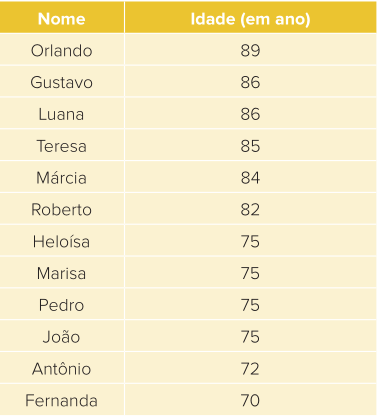
\includegraphics[scale=0.6]{imagens/enem-2020.png}
            \end{center} Nessas condições, a probabilidade de João ser a sétima pessoa do 
            grupo a receber sua restituição é igual a:

            \begin{enumerate}[label=(\alph*), noitemsep]
                \item {1}/{12}
                \item {7}/{12}
                \item {1}/{8}
                \item {5}/{6}
                \item {1}/{4}
            \end{enumerate}
        
        \novaquestao{Enem 2019}

            Em um determinado ano, os computadores da receita federal de um país identificaram 
            como inconsistentes 20\% das declarações de imposto de renda que lhe foram 
            encaminhadas. Uma declaração é classificada como inconsistente quando apresenta 
            algum tipo de erro ou conflito nas informações prestadas. Essas declarações 
            consideradas inconsistentes foram analisadas pelos auditores, que constataram 
            que 25\% delas eram fraudulentas. Constatou-se ainda que, dentre as declarações 
            que não apresentaram inconsistências, 6,25\% eram fraudulentas. Qual é a probabilidade 
            de, nesse ano, a declaração de um contribuinte ser considerada inconsistente, dado 
            que ela era fraudulenta?

            \begin{enumerate}[label=(\alph*), noitemsep]
                \item 0,0500
                \item 0,1000
                \item 0,1125
                \item 0,3125
                \item 0,5000
            \end{enumerate}
        
        \novaquestao{Enem 2017}

            Um morador de uma região metropolitana tem 50\% de probabilidade de atrasar-se 
            para o trabalho quando chove na região; caso não chova, sua probabilidade de 
            atraso é de 25\%. Para um determinado dia, o serviço de meteorologia estima em 
            30\% a probabilidade da ocorrência de chuva nessa região. Qual é a probabilidade 
            de esse morador se atrasar para o serviço no dia para o qual foi dada a 
            estimativa de chuva?

            \begin{enumerate}[label=(\alph*), noitemsep]
                \item 0,075
                \item 0,150
                \item 0,325
                \item 0,600
                \item 0,800
            \end{enumerate}
        
        \novaquestao{Enem PPL 2020}

            Para um docente estrangeiro trabalhar no Brasil, ele necessita validar o seu 
            diploma junto ao Ministério da Educação. Num determinado ano, somente para 
            estrangeiros que trabalharão em universidades dos estados de São Paulo e 
            Rio de Janeiro, foram validados os diplomas de 402 docentes estrangeiros. Na 
            tabela, está representada a distribuição desses docentes estrangeiros, por países
            de origem, para cada um dos dois estados.

            \begin{center}
                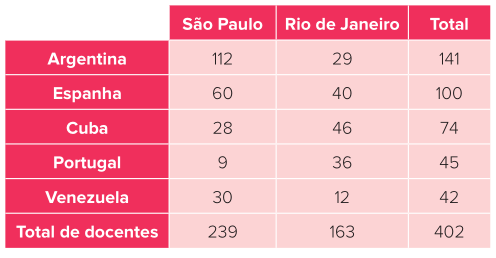
\includegraphics[scale=0.5]{imagens/enem-ppl-2020.png}
            \end{center} A probabilidade de se escolher, aleatoriamente, um docente espanhol, 
            sabendo-se que ele trabalha em uma universidade do estado de São Paulo é:

            \begin{enumerate}[label=(\alph*), noitemsep]
                \item {60}/{402}
                \item {60}/{239}
                \item {60}/{100}
                \item {100}/{239}
                \item {279}/{402}
            \end{enumerate}
        
        \novaquestao{Enem PPL 2018}
            
            O gerente de uma empresa sabe que 70\% de seus funcionários são do sexo 
            masculino e foi informado de que a porcentagem de empregados fumantes nessa 
            empresa é de 5\% dos homens e de 5\% das mulheres. Selecionando, ao acaso, a ficha 
            de cadastro de um dos funcionários, verificou tratar-se de um fumante. Qual 
            a probabilidade de esse funcionário ser do sexo feminino?

            \begin{enumerate}[label=(\alph*), noitemsep]
                \item 50,0\%
                \item 30,0\%
                \item 16,7\%
                \item 5,0\%
                \item 1,5\%
            \end{enumerate}
        
        \novaquestao{Enem 2020}

            Um apostador deve escolher uma entre cinco moedas ao acaso e lançá-la sobre uma 
            mesa, tentando acertar qual resultado (cara ou coroa) sairá na face superior da 
            moeda. Suponha que as cinco moedas que ele pode escolher sejam diferentes:

            \begin{itemize}
                \item duas delas têm “cara” nas duas faces;
                \item uma delas tem “coroa” nas duas faces;
                \item duas delas são normais (cara em uma face e coroa na outra).
            \end{itemize} Nesse jogo, qual é a probabilidade de o apostador obter uma face 
            “cara” no lado superior da moeda lançada por ele?

            \begin{enumerate}[label=(\alph*), noitemsep]
                \item {1}/{8}
                \item {2}/{5}
                \item {3}/{5}
                \item {3}/{4}
                \item {4}/{5}
            \end{enumerate}

        \novaquestao{UEA SIS II 2021}

            Um dado honesto de seis faces, numeradas de 1 a 6, será
            lançada três vezes. Sendo $S$ a soma dos números obtidos
            nesses três lançamentos, a probabilidade de a soma $S$ ser 
            igual a 15 ou igual a 16 é:

            \begin{enumerate}[label=(\alph*), noitemsep]
                \item {1}/{27}
                \item {2}/{27} %
                \item {1}/{9}
                \item {2}/{9}
                \item {1}/{2}
            \end{enumerate}

        \novaquestao{UEA SIS II 2021}

            Melissa e Janaína compraram, independentemente uma da
            outra, ingressos para uma mesma sessão de cinema. Se os
            assentos que elas compraram estão na fileira G, que possui 10
            assentos lado a lado, a probabilidade de que as duas sentem-se
            uma ao lado da outra é:

            \begin{enumerate}[label=(\alph*), noitemsep]
                \item 5\%
                \item 10\%
                \item 15\%
                \item 20\%  %
                \item 25\%
            \end{enumerate}

        \novaquestao{UEA MACRO 2020}

            Em uma urna, há 16 bolas numeradas de \textbf{21 a 36}.
            Retirando-se aleatoriamente uma bola dessa urna, a probabilidade
            de que a soma dos algarismo da bola sorteada seja divisível por 4 é:

            \begin{enumerate}[label=(\alph*), noitemsep]
                \item {1}/{2}
                \item {3}/{8}
                \item {3}/{16}
                \item {1}/{4}  %
                \item {5}/{16}
            \end{enumerate}

        \novaquestao{UEA SIS II 2017}

            Ana e Beatriz são alunas de uma classe onde foram sorteados
            dois livros para dois estudantes diferentes. Essa classe tem 10
            meninas e 12 meninos e no primeiro sorteio saiu o nome de Ana. Ao
            sortear o segundo nome, a professora avisou que era de uma menina
            e Beatriz calculou corretamente que a probabilidade de ter sido ela
            a sorteada era:

            \begin{enumerate}[label=(\alph*), noitemsep]
                \item {1}/{3}
                \item {1}/{5}
                \item {1}/{8}
                \item {1}/{9}  %
                \item {1}/{10}
            \end{enumerate}

        \novaquestao{UEA SIS II 2012}

            Em um cesto há 250 camu-camus, dos quais 20\% estão verdes
            e 500 acerolas, das quais 15\% também estão verdes. Se uma pessoa
            retirar ao acaso um fruto desses cesto, a probabilidade de que o 
            fruto esteja verde é:

            \begin{enumerate}[label=(\alph*), noitemsep]
                \item {2}/{3}
                \item {1}/{3}
                \item {1}/{4}
                \item {1}/{5}  
                \item {1}/{6} %
            \end{enumerate}

        \novaquestao{UEA MACRO 2012}

            Uma lanchonete de Manaus oferece aos clientes um "combinado",
            composto de um sanduíche e um suco. Pode-se escolher, de forma independente,
            entre dois tipos de sanduíche e três tipos de suco. A experiência
            mostra que 30\% dos clientes comem x-caboquinho simples (fatias de queijo
            coalho e lascas de tucumã no pão francês) e os restantes a sua versão
            mais refinada, que leva também fatias de banana frita. Por outro lado,
            20\% deles pedem suco de cupuaçu, 30\% suco de maracujá e os restantes suco
            de manga. Nessas condições, a probabilidade de que um cliente peça 
            x-caboquinho simples e suco de manga é:

            \begin{enumerate}[label=(\alph*), noitemsep]
                \item 35\%
                \item 15\% %
                \item 65\%
                \item 80\%  
                \item 40\%
            \end{enumerate}

        \novaquestao{UEA MACRO 2022}

            A comissão técnica de um time de basquete constatou que um
            determinado jogador, ao efetuar dois lances livres, um após o outro,
            tem probabilidades diferentes de acerto. A probabilidade de acertar
            o primeiro lance é de {2}/{3} e a probabilidade de acertar o segundo lance
            é de {2}/{5}, independentemente do resultado do primeiro lance. Nessas
            condições, a probabilidade desse jogador acertar o primeiro lance e 
            não acertar o segundo é de:

            \begin{enumerate}[label=(\alph*), noitemsep]
                \item {1}/{5}
                \item {2}/{5} %
                \item {1}/{15}
                \item {2}/{15} 
                \item {2}/{3}
            \end{enumerate}
        
        \novaquestao{UEA SIS II 2016}
            
            Em uma urna há 20 bolas numeradas de 20 a 39. Retirando-se aleatoriamente
            uma bola dessa urna, a probabilidade de que o número da bola seja múltiplo
            de 3 e que a soma dos algarismos seja menor ou igual a 7 é:

            \begin{enumerate}[label=(\alph*), noitemsep]
                \item {3}/{5}
                \item {2}/{5} 
                \item {1}/{5} %
                \item {3}/{20} 
                \item {1}/{20}
            \end{enumerate}

    \section*{Questões adicionais}

        \novaquestao{EEAR 2005}

            Seja $A = \left\{k_1, k_2, k_3, k_4, k_5\right\}$. o espaço amostral de um experimento aleatório. 
            Considere a seguinte:$ P(k_1)={1}/{8},\ P(k_2)={1}/{10},\ P(k_3)={2}/{5},\ P(k_4)=x$. O 
            valor de $x$ é:

            \begin{enumerate}[label=(\alph*), noitemsep]
                \item 36,5\%
                \item 37\%
                \item 37,25\%
                \item 37,5\%    %
                \item 38\%
            \end{enumerate}
        
        \novaquestao{EEAR 2007}

            Cinco casais (marido e mulher) estão juntos em um restaurante. 
            Escolhendo 2 pessoas ao acaso, a probabilidade de termos um marido e sua mulher é:

            \begin{enumerate}[label=(\alph*), noitemsep]
                \item {1}/{9}
                \item {1}/{10} %
                \item {1}/{11}
                \item {1}/{12}
                \item {1}/{13}
            \end{enumerate}
        
        \novaquestao{EEAR 2008}

            Uma urna contém 3 bolas verdes e 4 amarelas. Ao retirar, sem reposição, duas bolas, 
            a probabilidade delas serem amarelas é:

            \begin{enumerate}[label=(\alph*), noitemsep]
                \item {2}/{7}
                \item {3}/{7}
                \item {4}/{7}
                \item {6}/{7}
                \item {5}/{7}
            \end{enumerate}

        \novaquestao{EEAR 2016}

            Em um lançamento simultâneo de dois dados, sabe-se que ocorreram 
            somente números diferentes de 1 e 4. A probabilidade de o produto formado por esses 
            dois números ser par é:

            \begin{enumerate}[label=(\alph*), noitemsep]
                \item {1}/{2}
                \item {3}/{4} %
                \item {3}/{5}
                \item {7}/{12}
                \item {13}/{12}
            \end{enumerate}

        \novaquestao{EEAR 2003}

            No lançamento simultâneo de dois dados perfeitos, a probabilidade de obter 
            soma diferente de 11 é, aproximadamente,

            \begin{enumerate}[label=(\alph*), noitemsep]
                \item 5,5\%
                \item 94,4\%  %
                \item 83,4\%
                \item 16,6\%
                \item 13\%
            \end{enumerate}


        
        \novaquestao{UEG-GO 2019}
            
            Em um programa de televisão, será sorteado um dos participantes para executar 
            determinada tarefa. Sabe-se que, entre os participantes, 4 são homens, 6 são 
            mulheres e uma mulher recebeu imunidade e não poderá participar do sorteio. 
            Colocando-se os nomes dos participantes que serão sorteados em uma urna e 
            retirando-se um deles ao acaso, a probabilidade de que seja uma mulher é de:

            \begin{enumerate}[label=(\alph*), noitemsep]
                \item {1}/{2}
                \item {1}/{5}
                \item {3}/{5} 
                \item {1}/{9} 
                \item {5}/{9}
            \end{enumerate}
        
        \novaquestao{UFRR 2024}
            Um dado honesto, com 6 faces numeradas de 1 a 6, é lançado duas vezes. 
            Qual é a probabilidade de se obter, nas faces voltadas para cima, números 
            que somados resultam um número ímpar menor do que 7?

            \begin{enumerate}[label=(\alph*), noitemsep]
                \item {1}/{6}
                \item {1}/{9}
                \item {2}/{3} 
                \item {1}/{12} 
                \item {1}/{4}
            \end{enumerate}
        
        \novaquestao{UFU-MG 2018}

            As irmãs Ana e Beatriz e seus respectivos namorados vão sentar-se em um banco de 
            jardim (figura) de modo que cada namorado fique ao lado de sua namorada.

            \begin{center}
                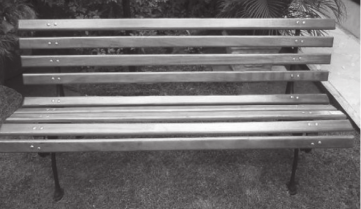
\includegraphics[scale=0.6]{imagens/ufu-2018.png}
            \end{center} A probabilidade de as irmãs sentarem-se uma ao lado da outra é igual a:

            \begin{enumerate}[label=(\alph*), noitemsep]
                \item 0,25
                \item 0,33
                \item 0,45
                \item 0,50
                \item 0,75
            \end{enumerate}
        
        \novaquestao{ESPM-SP 2019}

            Uma urna contém 5 bolas idênticas numeradas de 1 a 5. Quatro bolas serão retiradas
            uma a uma, aleatoriamente, dessa urna e enfileiradas em uma canaleta da esquerda 
            para a direita, na ordem de retirada, formando um número de 4 algarismos. A 
            probabilidade de o algarismo das unidades ser o maior de todos os algarismos 
            desse número é igual a:

            \begin{enumerate}[label=(\alph*), noitemsep]
                \item {1}/{6}
                \item {2}/{3}
                \item {1}/{2}
                \item {1}/{4}
                \item {1}/{3}
            \end{enumerate}
        
        \novaquestao{Unioeste-PR 2019}

            Uma empresa possui 10 diretores, dos quais, 3 são suspeitos de corrupção. Foi 
            resolvido se fazer uma investigação composta por uma comissão de 5 diretores da 
            empresa. A única condição imposta é que a comissão de investigação selecionada 
            tenha a maioria de diretores não suspeitos. Selecionada, ao acaso, uma comissão para 
            apuração das suspeitas formada por diretores desta empresa, é CORRETO afirmar que a 
            probabilidade de que esta comissão atenda à condição imposta está no intervalo:

            \begin{enumerate}[label=(\alph*), noitemsep]
                \item (0,01; 0,50)
                \item (0,50; 0,70)
                \item (0,70; 0,80)
                \item (0,80; 0,90)
                \item (0,90; 0,99)
            \end{enumerate}
        
        \novaquestao{Fuvest-SP 2018}
            
            Em uma urna, há bolas amarelas, brancas e vermelhas. Sabe-se que:

            \begin{enumerate}[label=\Roman*.]
                \item A probabilidade de retirar uma bola vermelha dessa urna é o dobro da 
                probabilidade de retirar uma bola amarela.
                \item Se forem retiradas 4 bolas amarelas dessa urna, a probabilidade de 
                retirar uma bola vermelha passa a ser {1}/{2}.
                \item Se forem retiradas 12 bolas vermelhas dessa urna, a probabilidade de 
                retirar uma bola branca passa a ser {1}/{2}
            \end{enumerate} A quantidade de bolas brancas na urna é:

            
            \begin{enumerate}[label=(\alph*), noitemsep]
                \item 8
                \item 10
                \item 12
                \item 14
                \item 16
            \end{enumerate}
        
        \novaquestao{UFVJM-MG 2022}

            Pedro e Paula participam de um grupo de dez voluntários, dentre os quais três 
            serão sorteados para participarem de um teste com uma nova vacina. A probabilidade 
            de pelo menos um dos dois ser sorteado é de:

            \begin{enumerate}[label=(\alph*), noitemsep]
                \item {4}/{15}
                \item {7}/{15}
                \item {8}/{15}
                \item {11}/{15}
                \item {13}/{15}
            \end{enumerate}
        
        \novaquestao{FGV-SP 2022}

            Em um trecho retilíneo de uma rua há 14 vagas, lado a lado, demarcadas para o 
            estacionamento de carros. Os carros entram e saem aleatoriamente dessas vagas e 
            em um dado momento havia 9 carros estacionados. A probabilidade, nesse momento, 
            de não haver vagas vazias lado a lado é de:


            \begin{enumerate}[label=(\alph*), noitemsep]
                \item {1}/{24}
                \item {5}/{24}
                \item {3}/{40}
                \item {9}/{125}
                \item {18}/{143}
            \end{enumerate}
        
        \novaquestao{UPE/SSA 2016}

            Se dois dados idênticos e não viciados são lançados, a probabilidade de a soma 
            dos pontos obtidos ser um múltiplo de 2 ou um múltiplo de 3 é de aproximadamente:


            \begin{enumerate}[label=(\alph*), noitemsep]
                \item $66,6 \%$
                \item $60,0 \%$
                \item $55,2 \%$
                \item $35,3 \%$
                \item $33,0 \%$
            \end{enumerate}
        
        \novaquestao{UERJ 2018}
            
            Um jogo consiste em lançar cinco vezes um dado cúbico, cujas faces são numeradas 
            de 1 a 6, cada uma com a mesma probabilidade de ocorrer. Um jogador é considerado 
            vencedor se obtiver pelo menos três resultados pares. A probabilidade de um jogador 
            vencer é:

            \begin{enumerate}[label=(\alph*), noitemsep]
                \item {3}/{5}
                \item {2}/{3}
                \item {1}/{5}
                \item {1}/{2}
                \item {3}/{2}
            \end{enumerate}
        
        \novaquestao{Efomm-RJ 2016}

            Um dado cúbico, não viciado, com faces numeradas de 1 a 6, é lançado três vezes. 
            Em cada lançamento, anota-se o número obtido na face superior do dado, formando-se
            uma sequência (a, b, c). Qual é a probabilidade de que b seja sucessor de a e 
            que c seja sucessor de b OU que a, b, e c sejam primos?

            \begin{enumerate}[label=(\alph*), noitemsep]
                \item {4}/{216}
                \item {27}/{216}
                \item {108}/{216}
                \item {31}/{216}
                \item {10}/{216}
            \end{enumerate}
        
        \novaquestao{Unicamp-SP 2018}
            
            Lançando-se determinada moeda tendenciosa, a probabilidade de sair cara é o 
            dobro da probabilidade de sair coroa. Em dois lançamentos dessa moeda, a 
            probabilidade de sair o mesmo resultado é igual a:

            \begin{enumerate}[label=(\alph*), noitemsep]
                \item {1}/{2}
                \item {5}/{9}
                \item {2}/{3}
                \item {3}/{5}
                \item {9}/{5}
            \end{enumerate}
        
        
        
        \novaquestao{Mackenzie-SP 2017}
            
            João guardou as duas chaves de sua casa em uma caixa que estava na estante 
            da sala. Ao sair, no dia seguinte, foi pegar as chaves de casa na caixa em 
            que as havia guardado e percebeu que a caixa continha 5 chaves e não apenas as 
            duas que eram suas. Como não conseguia distinguir as suas chaves e já estava 
            atrasado para um compromisso, João resolveu sortear 3 das 5 chaves e levá-las 
            consigo. Assim, a probabilidade de que João consiga entrar em casa quando 
            voltar é:

            \begin{enumerate}[label=(\alph*), noitemsep]
                \item 0,5
                \item 0,7
                \item 0,9
                \item 0,6
                \item 0,4
            \end{enumerate}
        
        \novaquestao{EsPCEx-SP 2020}

            Numa sala existem duas caixas com bolas amarelas e verdes. Na caixa 1, há 3 
            bolas amarelas e 7 bolas verdes. Na caixa 2, há 5 bolas amarelas e 5 bolas 
            verdes. De forma aleatória, uma bola é extraída da caixa 1, sem que se saiba 
            a sua cor, e é colocada na caixa 2. Após esse procedimento, a probabilidade 
            de extrair uma bola amarela da caixa 2 é igual a:

            \begin{enumerate}[label=(\alph*), noitemsep]
                \item {49}/{110}
                \item {51}/{110}
                \item {53}/{110}
                \item {57}/{110}
                \item {61}/{110}
            \end{enumerate}
        
        \novaquestao{Unesp 2017}

            Em um jogo de tabuleiro, o jogador desloca seu peão nas casas por meio dos pontos 
            obtidos no lançamento de um par de dados convencionais e não viciados. Se o jogador
            obtém números diferentes nos dados, ele avança um total de casas igual à soma dos
            pontos obtidos nos dados, encerrando-se a jogada. Por outro lado, se o jogador 
            obtém números iguais nos dados, ele lança novamente o par de dados e avança seu 
            peão pela soma dos pontos obtidos nos dois lançamentos, encerrando-se a jogada. A
            figura a seguir indica a posição do peão no tabuleiro desse jogo antes do início 
            de uma jogada.

            \begin{center}
                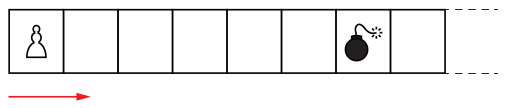
\includegraphics[scale=0.5]{imagens/unesp-2017.png}
            \end{center} Iniciada a jogada, a probabilidade de que o peão encerre a jogada 
            na casa indicada na figura com a bomba é igual a:

            \begin{enumerate}[label=(\alph*), noitemsep]
                \item {37}/{324}
                \item {49}/{432}
                \item {23}/{144}
                \item {23}/{135}
                \item {23}/{216}
            \end{enumerate}
        
        \novaquestao{UFRGS 2018}

            Considere os números naturais de 1 até 100. Escolhido ao acaso um desses números, 
            a probabilidade de ele ser um quadrado perfeito é:

            \begin{enumerate}[label=(\alph*), noitemsep]
                \item {1}/{10}
                \item {4}/{25}
                \item {3}/{10}
                \item {1}/{2}
                \item {9}/{10}
            \end{enumerate}
        
        \novaquestao{FMJ-SP 2024}
            
            Uma campanha publicitária irá distribuir 400 ingressos para um espetáculo, sendo 
            120 ingressos especiais e os demais ingressos comuns. A distribuição dos ingressos
            será feita no estande da campanha, com os ingressos sendo depositados em uma urna 
            e cada interessado pegando aleatoriamente um ingresso. A probabilidade de o 
            primeiro ingresso especial ser retirado pela segunda pessoa a pegar um ingresso 
            é:

            \begin{enumerate}[label=(\alph*), noitemsep]
                \item {3}/{10}
                \item {3}/{5}
                \item {4}/{19}
                \item {1}/{12}
                \item {2}/{15}
            \end{enumerate}
        
        \novaquestao{UFPR 2021}

            Ana, Beatriz e Carlos pediram uma pizza de oito fatias, metade sabor mozarela e 
            outra metade sabor calabresa. Sabendo que Ana e Carlos preferem calabresa e 
            Beatriz prefere mozarela, após cada um dos três ter escolhido uma fatia de pizza 
            de acordo com sua preferência, qual é a probabilidade de Ana, Beatriz e Carlos 
            terem escolhido pedaços que estejam lado a lado na \textit{pizza}?

            \begin{enumerate}[label=(\alph*), noitemsep]
                \item {1}/{12}
                \item {1}/{6}
                \item {1}/{4}
                \item {1}/{3}
                \item {1}/{2}
            \end{enumerate}

        \novaquestao{AFA 1999}

            A probabilidade de observarmos um número na face superior de um 
            dado viciado é diretamente proporcional a esse número. Ao lançarmos esse dado, 
            a probabilidade de ocorrer um número par é:

            \begin{enumerate}[label=(\alph*), noitemsep]
                \item {1}/{2}
                \item {11}/{21}
                \item {4}/{7}
                \item {13}/{21}
                \item {12}/{21}
            \end{enumerate}

        \novaquestao{PUC-Rio 2011}
            
            Um móvel tem três gavetas iguais. Em uma gaveta há duas bolas brancas, em outra há duas bolas pretas, e na terceira há uma bola 
            branca e outra preta. Abrimos uma gaveta ao acaso e tiramos uma bola ao acaso sem olhar a segunda bola que está na gaveta. 
            A bola que tiramos é branca. Qual é a probabilidade de que a segunda bola que ficou sozinha na gaveta seja também branca?

            \begin{enumerate}[label=(\alph*), noitemsep]
                \item {1}/{4}
                \item {1}/{3}
                \item {1}/{2} 
                \item {2}/{3} %
                \item {3}/{4}
            \end{enumerate}

        
        \novaquestao{ITA-SP 2021}
            
            Um dodecaedro regular tem 12 faces que são pentágonos regulares. Escolhendo-se 2 
            vértices distintos desse dodecaedro, a probabilidade de eles pertencerem a uma 
            mesma aresta é igual a:

            \begin{enumerate}[label=(\alph*), noitemsep]
                \item {15}/{100}
                \item {3}/{19}
                \item {15}/{190}
                \item {5}/{12}
                \item {2}/{5}
            \end{enumerate}
        
        \novaquestao{ITA-SP 2018}

            São dadas duas caixas, uma delas contém três bolas brancas e duas pretas e a outra
            contém duas bolas brancas e uma preta. Retira-se, ao acaso, uma bola de cada caixa. 
            Se $P_{1}$ é a probabilidade de que pelo menos uma bola seja preta e $P_{2}$ a 
            probabilidade de as duas bolas serem da mesma cor, então $P_{1}+P_{2}$ vale:


            \begin{enumerate}[label=(\alph*), noitemsep]
                \item {8}/{15}
                \item {7}/{15}
                \item {6}/{15}
                \item 1
                \item {17}/{15}
            \end{enumerate}
        

    \end{multicols}
    
\end{document}